\chapter{Cronograma}
\label{chap:cronograma}

\begin{figure}[!htb]
    \centering
    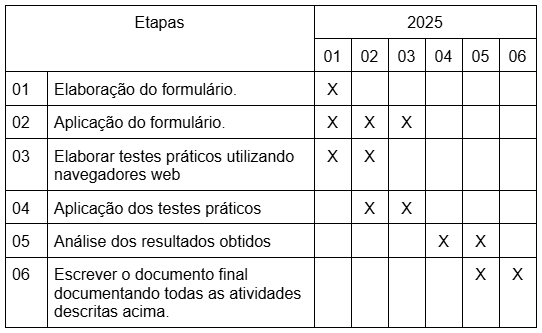
\includegraphics[width=0.85\linewidth]{assets/cronograma.png}
    \label{fig:cronograma}
\end{figure}

O planejamento acima, atribui atividades essenciais para o progresso do TCC ao longo de um período de oito meses. Esta é uma abordagem bem estruturada e organizada. A definição clara das fases permite que cada objetivo específico contribua de forma incremental para o avanço do projeto, para garantir uma construção contínua e coerente do trabalho acadêmico. 

Outro resultado da cuidadosa estruturação do horário é que este não só permitirá uma gestão eficiente do tempo e dos demais recursos disponíveis, como também facilitará o acompanhamento do cumprimento dos prazos e da realização das tarefas. Dessa forma, cada fase do projeto é estruturada, o que minimiza riscos de atrasos e retrabalhos e promove processos produtivos e aderência aos requisitos acadêmicos estabelecidos.